\documentclass[color]{csbulletin}[2021/03/19] % version requirement
\renewcommand\cslogodir{.} % Directory with logos, pictures, etc.
\usepackage[utf8]{inputenc}

% Podpora pro hyperlinky
\makeatletter
\ifcsbul@web
  \usepackage[implicit=false, hidelinks]{hyperref}
  \usepackage{pax}
  \usepackage{etoolbox}
  \preto\csbul@PDF@clanek{%
    \hypertarget{page.\thepage}{}%
  }{}{}
  \def\l@clanek#1#2{%
    {%
      \let\protect\@unexpandable@protect
      \immediate\write\zw@engtoc{%
        \protect\contentsline{clanek}{#1}{#2}%
      }%
    }%
    \@dottedtocline{-2}{\z@}{2em}{%
      \hyperlink{page.#2}{#1}%
    }{%
      \hyperlink{page.#2}{#2}%
    }%
  }
\fi
\makeatother

% Macros in the .toc output files
\def\boolfalse#1{}
\def\defcounter#1#2{}
\makeatletter
\DeclareRobustCommand{\La}{L\kern-.36em%
        {\sbox\z@ T%
         \vbox to\ht\z@{\hbox{\check@mathfonts
                              \fontsize\sf@size\z@
                              \math@fontsfalse\selectfont
                              A}%
                        \vss}%
        }}
\makeatother
\def\AllTeX{(\La\kern-.075em)\kern-.075em\TeX}

\usepackage{alltt}
\errorcontextlines 999

\rok{2023}
\cislo{3--4}
\doisufix{2023-3-4/\thepage}
\uzaverka 30.11.2023  %
\naklad{250}
\CSBULilustrace{Jan Šustek}
\makeatletter
  \bul@rr@toks{%
    Redakční rada:        & Pavel Haluza, Lukáš Novotný, Vít Starý Novotný, \\
                          & Michal Růžička a Jan Šustek (šéfredaktor) \\
    Vědecká rada:         & Ján Buša (předseda), Jiří Demel, Jaromír Kuben \\
                          & (zástupce předsedy), Jiří Rybička a Petr Sojka \\
    Technická redakce:    & Vít Starý Novotný \\
    Jazyková korektura:   & Zbyněk Michálek \\
    Evidenční číslo MK:   & E 7629 \\
  }
\makeatother

\usepackage{url}
\begin{document}

\catcode`\^7 % vyřazení shortcutu ze slovenského babelu
\shorthandoff{-} % vyřazení shortcutu z českého babelu

% Makro \Obalka má v hranatých závorkách kód pro vložení obrázku, bez hranatých závorek
% má obálka jen prázdný rámeček
% Pro centrování jsou k dispozici makra \centerbox a \Centerbox
% definovaná v csbulobalka.sty
%

\makeatletter
\ifcsbul@web
  \Obalka[%
    \centering
    \begin{minipage}{64mm}%
      \raisebox{0mm}{%
        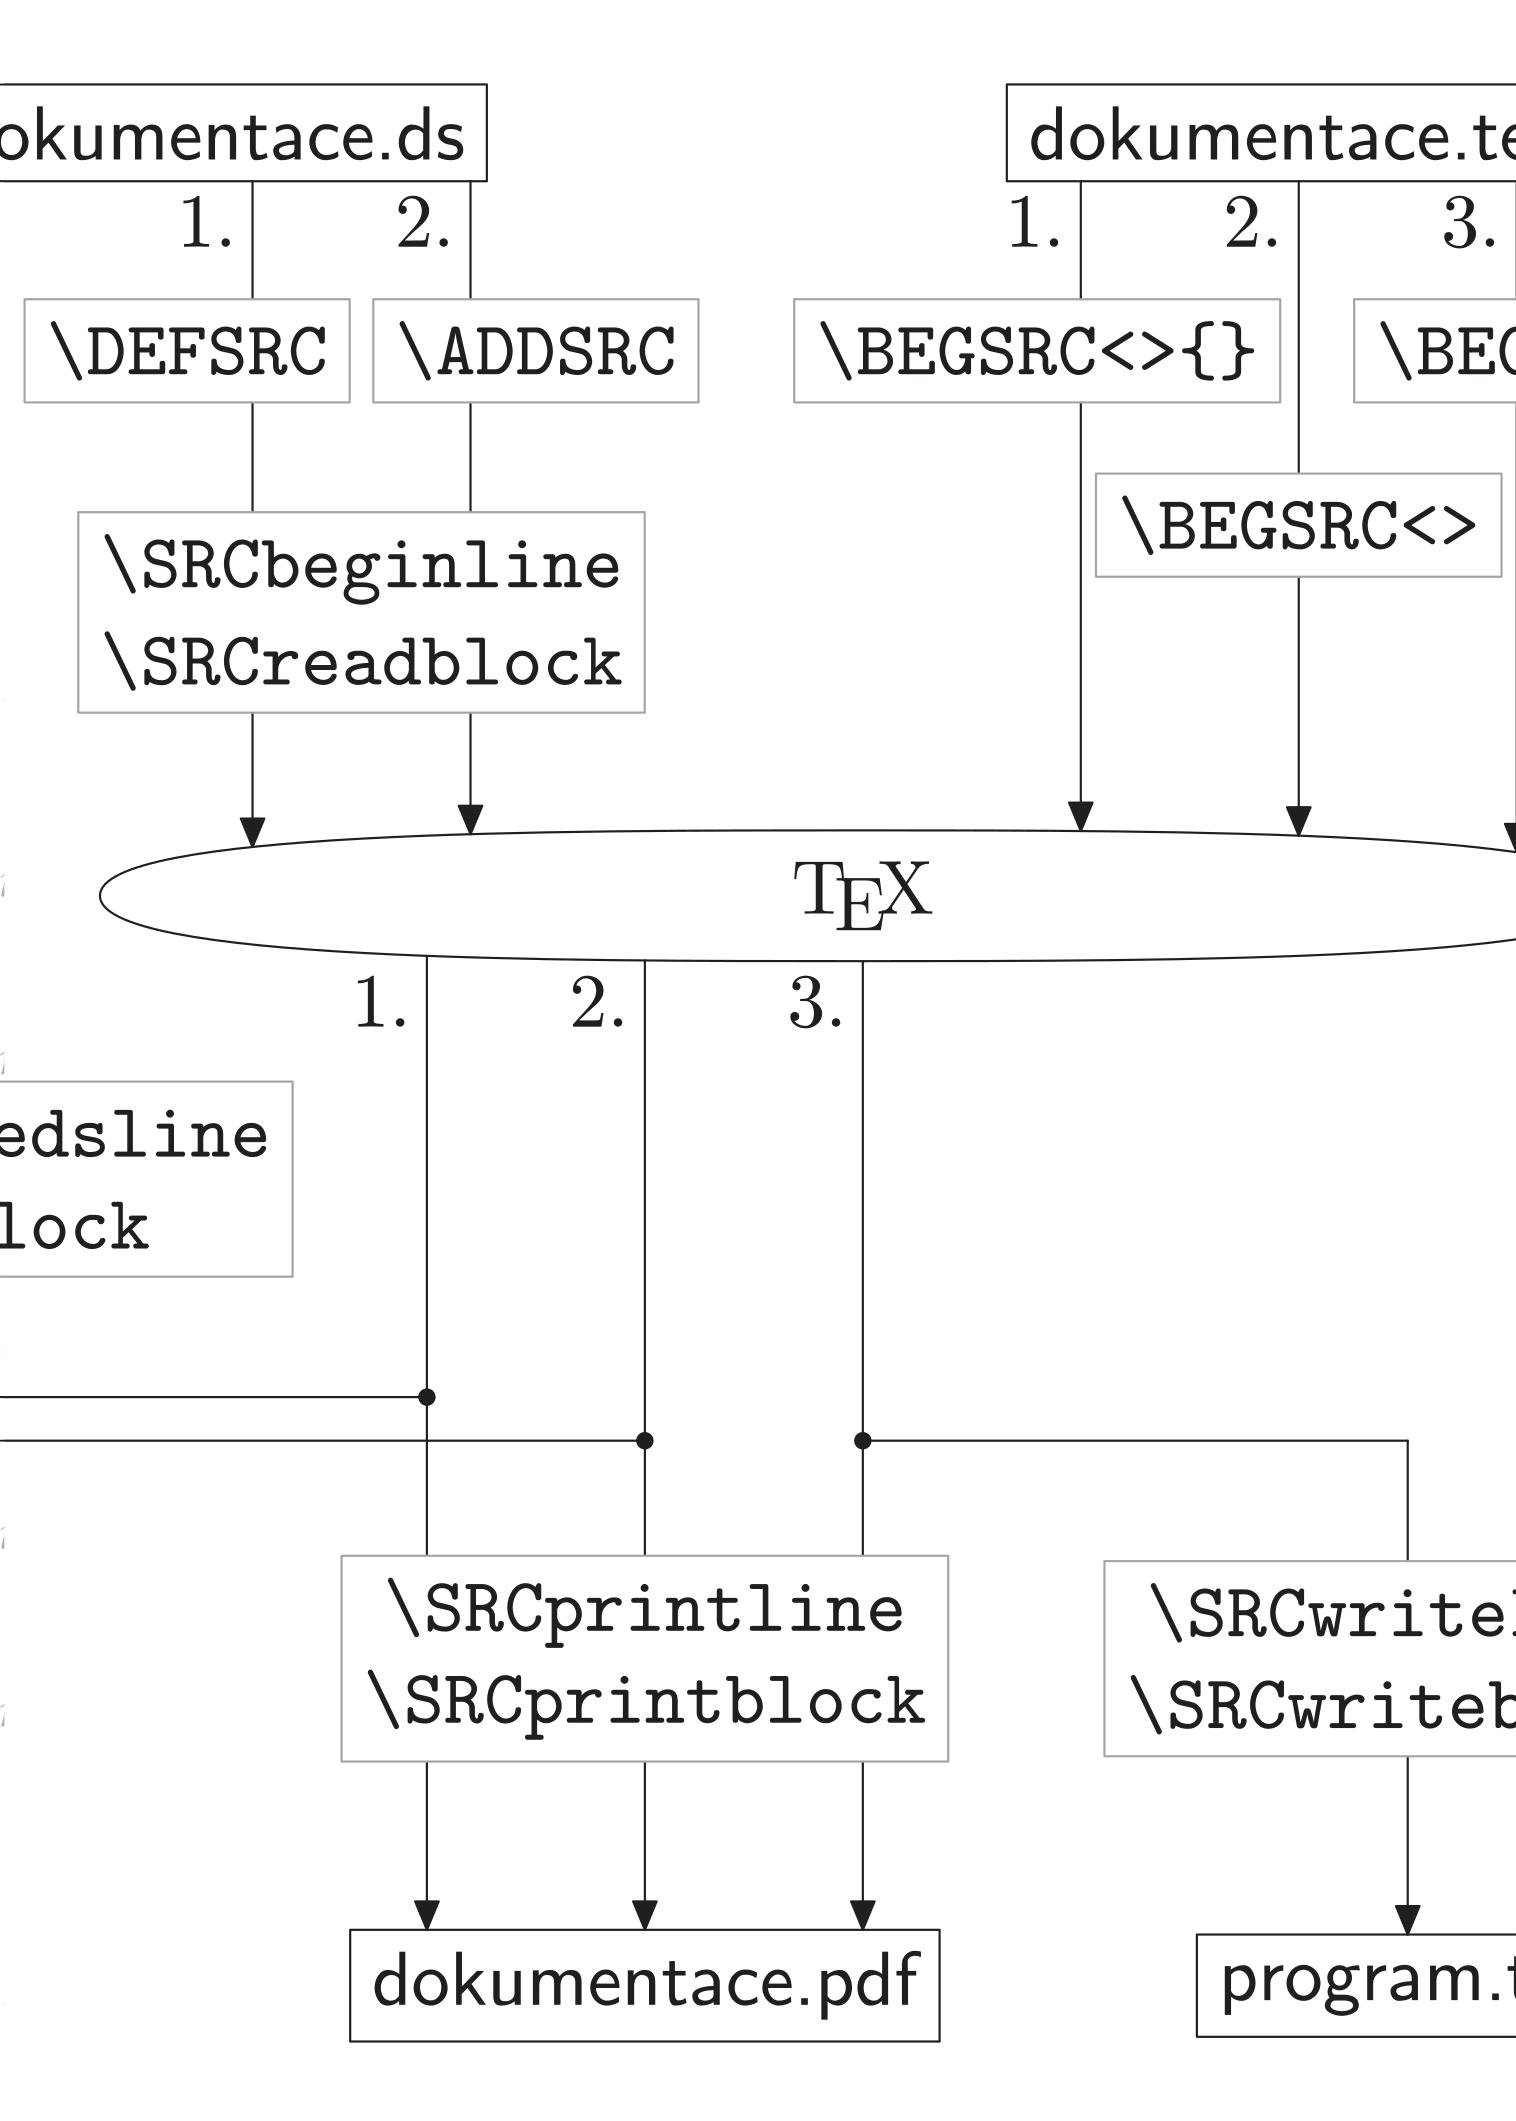
\includegraphics[
          width=\linewidth,
          trim={1.65cm 0 0.9cm 0},
          clip,
        ]{Sustek-literate-rezani/graf-1.pdf}%
      }%
    \end{minipage}%
  ]%
\else
  \Obalka[%
    \centering
    \begin{minipage}{64mm}%
      \raisebox{0mm}{%
        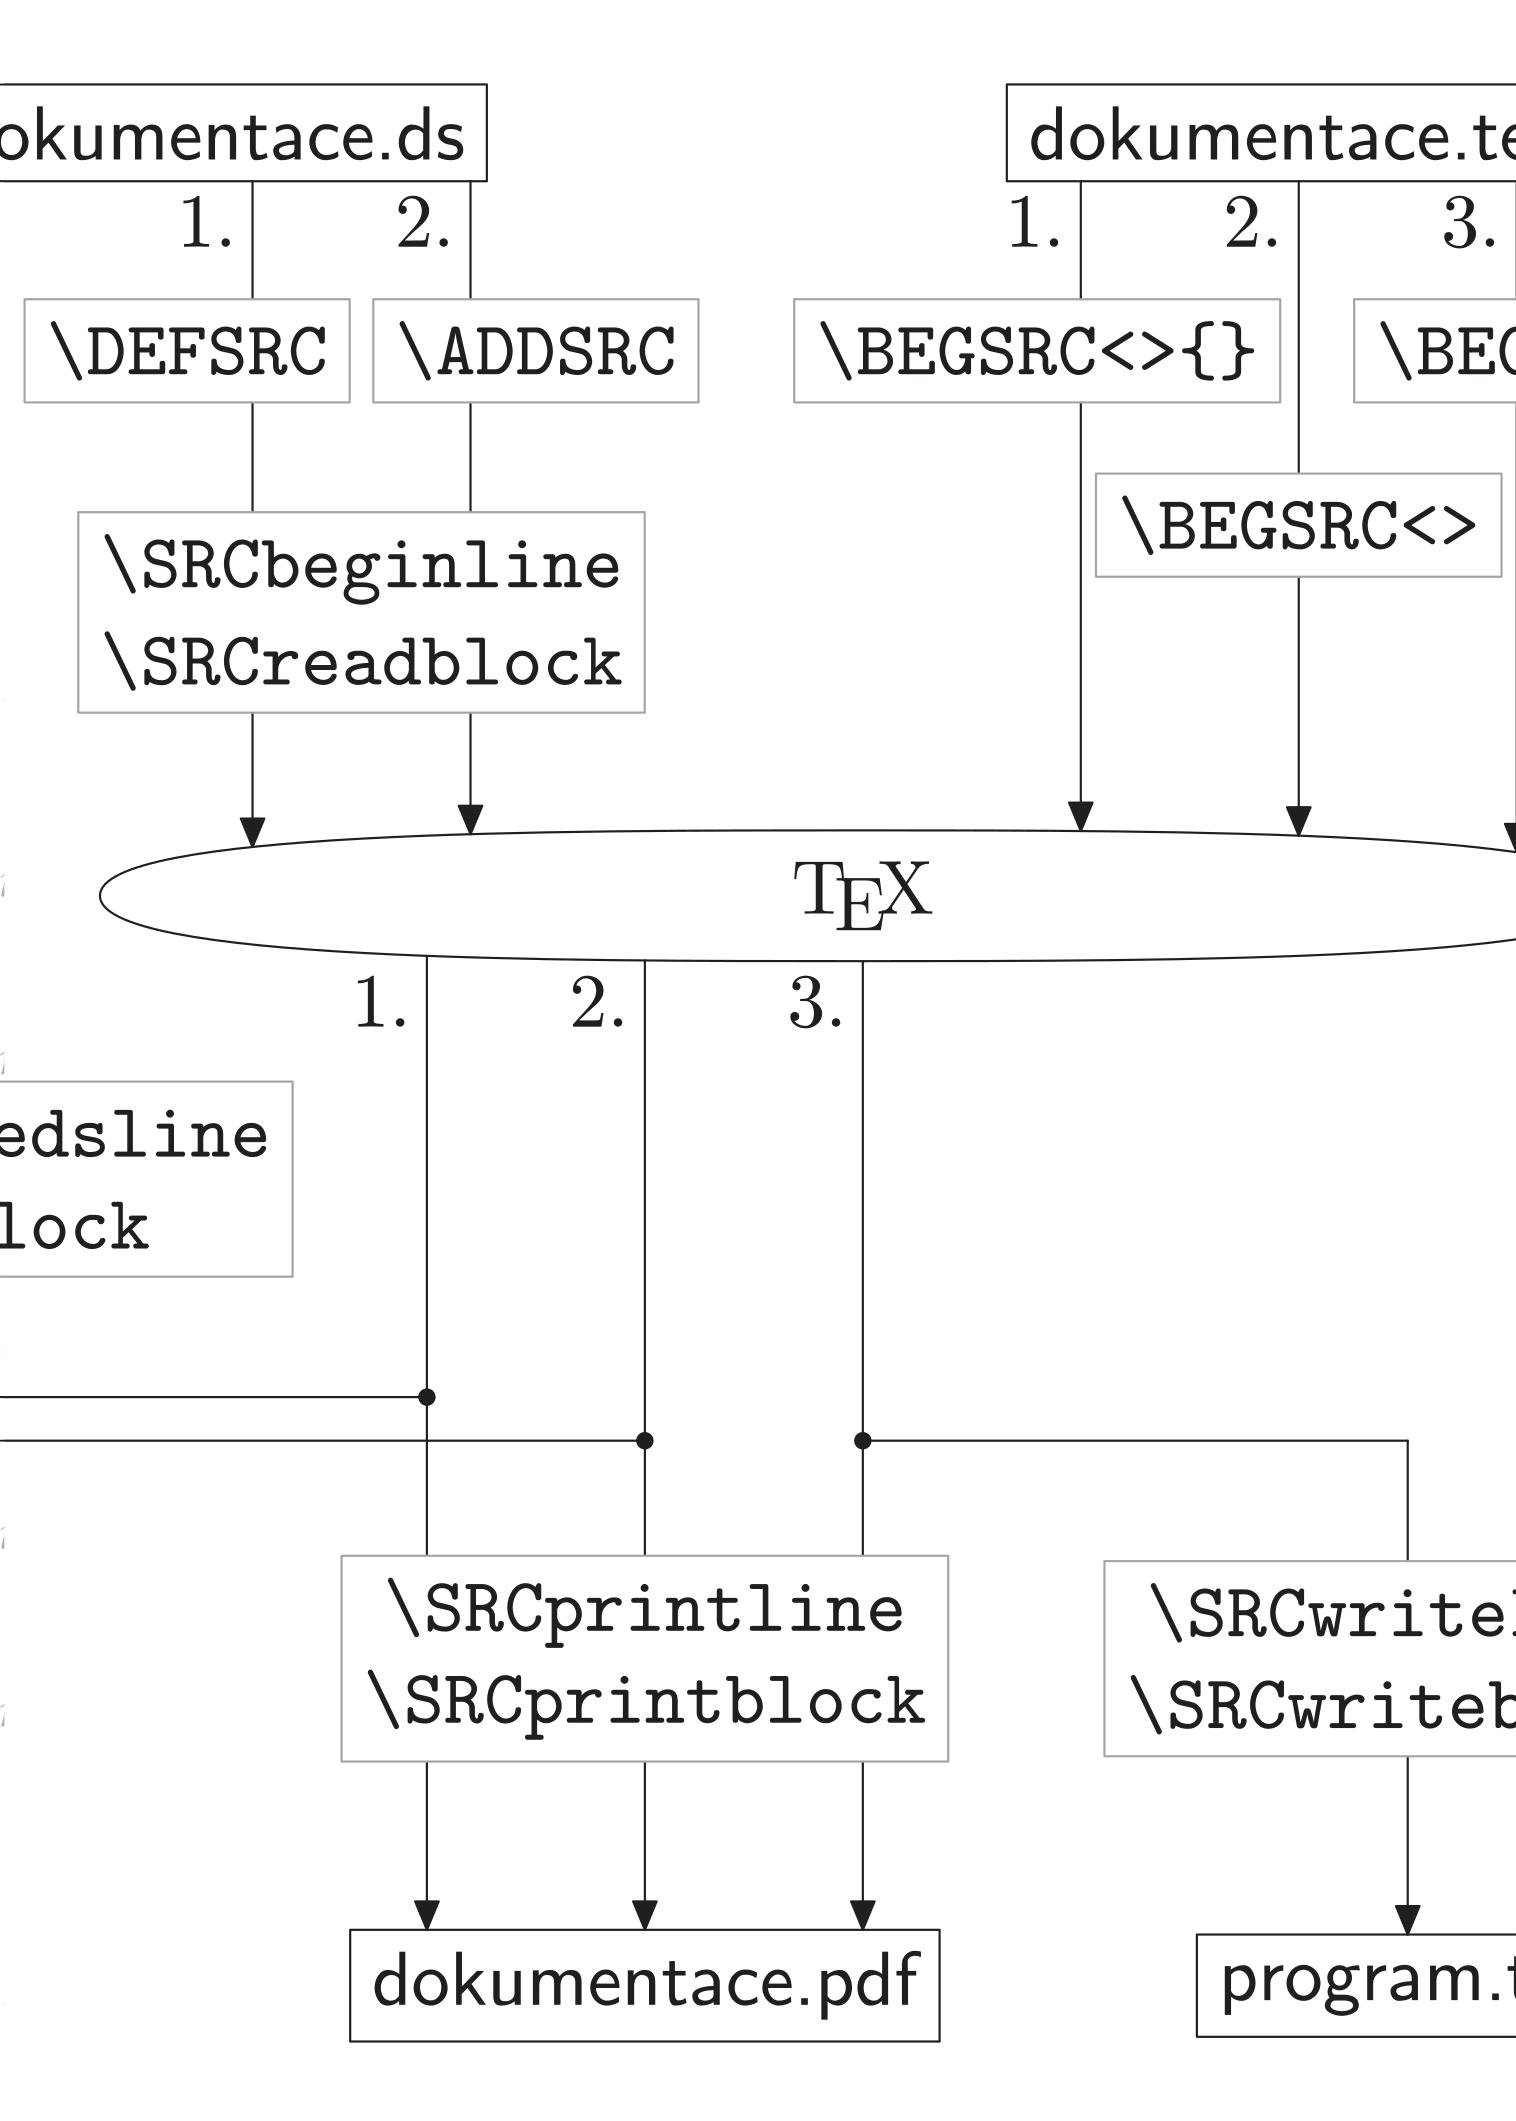
\includegraphics[
          width=\linewidth,
        ]{Sustek-literate-rezani/graf-1.png}%
      }%
    \end{minipage}%
  ]%
\fi
\makeatother

\begingroup
\hyphenpenalty=10000
\exhyphenpenalty=10000
\renewcommand\textls[2][]{#2}  % Zakážeme úpravy prokladu v textu nadpisů
\tableofcontents
\endgroup

\vfill
\begin{small}
\noindent
Zpravodaj Československého sdružení uživatelů \TeX u je vydáván v~tištěné podobě
a~distribuován zdarma členům sdružení. Vydaná čísla Zpravodaje v~elektronické
podobě (PDF) jsou bezodkladně veřejně vystavena na webové adrese
\texttt{https://www.cstug.cz/}\,.

\medskip\noindent
Své příspěvky do Zpravodaje můžete zasílat v~elektronické podobě, nejlépe jako
jeden archivní soubor \texttt{(.zip, .arj, .tar.gz)}, na e-mailovou adresu
\texttt{bulletin@cstug.cz}.
Nezapomeňte přiložit všechny soubory, které dokument načítá (s~výjimkou
standardních součástí \TeX~Live).
\end{small}

\bigskip

\noindent ISSN \ISSN\ (ti\v{s}t\v{e}n\'{a} verze)

\noindent ISSN \XISSN\ (online verze)


% \StartPage má v hranatých závorkách číslo první strany, default bez hranatých závorek je 1

\StartPage[61]

% template:
% \PDFclanek[adresar]{main}
% adresar = adresář (relativně) s článkem, musí to být podadresář aktuálního, jinak by skript
% nemusel správně pracovat
% main = jméno hlavního souboru bez přípony, přípona musí být .tex

\PDFclanek[StaryNovotny-uvodnik]{uvodnik}
\PDFclanek[StaryNovotny-tug]{main}
\PDFclanek[Sustek-literate-rezani]{literate}
\PDFclanek[Sustek-literate-rezani]{rezani}
\PDFclanek[StaryNovotny-markdown]{main}
\PDFclanek[Sojka-patterns]{main}
\PDFclanek[Beeton-newbie]{newbie}
\PDFclanek[StaryNovotny-l3seq]{main}

% tiráž
\tiraz

% anglický obsah
\begingroup
\hyphenpenalty=10000
\exhyphenpenalty=10000
\EnglishTOC
\endgroup

\end{document}
